\chapter{Asymptotic Analysis}
% Content for Chapter 4

\section*{\Large \textbf{Asymptotic Analysis}}

Asymptotic analysis is a method used to describe the behavior of functions as the input size \(n\) grows large. It provides a framework to compare algorithms by focusing on their dominant terms while ignoring constant factors and lower-order terms.

\subsection*{\large \textbf{1. Case Analysis}}

\begin{itemize}[leftmargin=2em]
  \item \textbf{Worst Case:} The maximum number of operations an algorithm performs on any input of size \(n\). This gives an upper bound.
  \item \textbf{Average Case:} The expected number of operations, averaged over all inputs of size \(n\) (assuming some probability distribution over inputs).
  \item \textbf{Best Case:} The minimum number of operations required for some input of size \(n\). Though fast, it is less useful for guarantees.
\end{itemize}

\subsection*{\large \textbf{2. Asymptotic Notations}}

\begin{itemize}[leftmargin=2em]
  \item \(\mathbf{O}\) \textbf{(Big-O):}  
  \(f(n) = O(g(n))\) if there exist constants \(c > 0\) and \(n_0 > 0\) such that  
  \[
    0 \le f(n) \le c \cdot g(n) \quad \text{for all } n \ge n_0.
  \]
  This is an upper bound on the growth rate of \(f(n)\).

  \item \(\mathbf{\Theta}\) \textbf{(Theta):}  
  \(f(n) = \Theta(g(n))\) if there exist constants \(c_1, c_2 > 0\) and \(n_0 > 0\) such that  
  \[
    0 \le c_1 \cdot g(n) \le f(n) \le c_2 \cdot g(n) \quad \text{for all } n \ge n_0.
  \]
  This provides a tight bound.

  \item \(\mathbf{\Omega}\) \textbf{(Big-Omega):}  
  \(f(n) = \Omega(g(n))\) if there exist constants \(c > 0\) and \(n_0 > 0\) such that  
  \[
    0 \le c \cdot g(n) \le f(n) \quad \text{for all } n \ge n_0.
  \]
  This is a lower bound on the growth rate.
\end{itemize}

\subsection*{\large \textbf{3. Graphical Representation}}

Below is a TikZ graph comparing the asymptotic bounds for the quadratic function \( f(n)=n^2 \). In this graph:
\begin{itemize}[leftmargin=2em]
  \item The red dashed curve represents an upper bound \( O(n^2) \) (e.g., \( 1.2\,n^2 \)).
  \item The blue solid curve represents a tight bound \( \Theta(n^2) \) (i.e., \( n^2 \)).
  \item The green dotted curve represents a lower bound \( \Omega(n^2) \) (e.g., \( 0.8\,n^2 \)).
\end{itemize}

\begin{figure}[H]
\centering
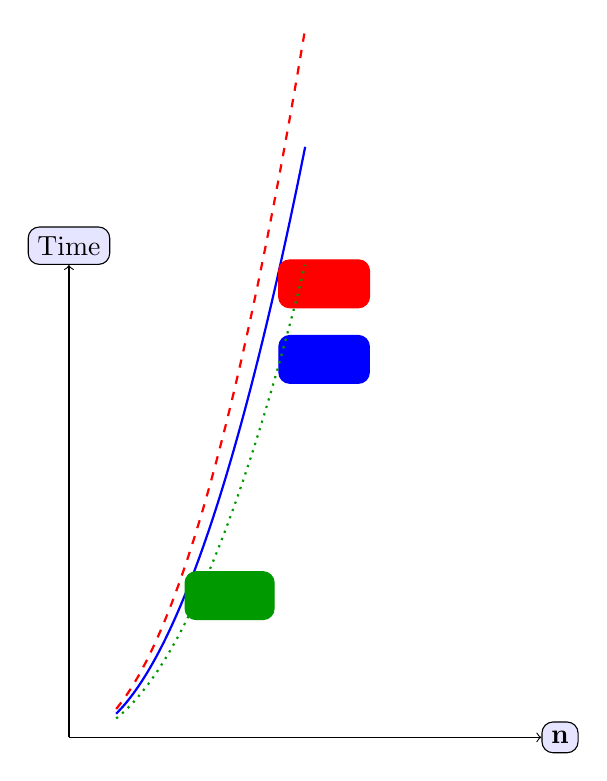
\begin{tikzpicture}[scale=1.2]
    % Axes
    \draw[->] (0,0) -- (5,0) node[right] {\(\mathbf{n}\)};
    \draw[->] (0,0) -- (0,5) node[above] {Time};
    
    % Theta(n^2): f(n) = n^2 (blue solid line)
    \draw[thick, blue, domain=0.5:2.5, smooth, variable=\x] plot ({\x}, {(\x*\x)});
    \node[blue] at (2.7,4) {\(\Theta(n^2)\)};
    
    % Big-O: f(n) = 1.2*n^2 (red dashed line)
    \draw[dashed, red, thick, domain=0.5:2.5, variable=\x] plot ({\x}, {1.2*(\x*\x)});
    \node[red] at (2.7,4.8) {\(O(n^2)\)};
    
    % Omega: f(n) = 0.8*n^2 (green dotted line)
    \draw[dotted, green!60!black, thick, domain=0.5:2.5, variable=\x] plot ({\x}, {0.8*(\x*\x)});
    \node[green!60!black] at (1.7,1.5) {\(\Omega(n^2)\)};
\end{tikzpicture}
\caption{Graphical illustration of \( O(n^2) \), \(\Theta(n^2)\), and \(\Omega(n^2)\).}
\end{figure}

\subsection*{\large \textbf{4. Example: Linear Search}}

Consider the Linear Search algorithm in an unsorted array of size \( n \).

\begin{itemize}[leftmargin=2em]
  \item \textbf{Best Case:} The key is found at the first index: \(\Theta(1)\).
  \item \textbf{Worst Case:} The key is found at the last index or not present: \( O(n) \).
  \item \textbf{Average Case:} On average, about \( \frac{n}{2} \) comparisons are made: \(\Theta(n)\).
\end{itemize}

\subsection*{\large \textbf{5. Additional C++ Examples}}

Below are two C++ examples that further illustrate algorithm behavior and their asymptotic analysis.

\subsubsection*{\textbf{Example 1: Binary Search}}

Binary Search on a sorted array runs in \( O(\log n) \) time. The following code snippet demonstrates the algorithm:

\begin{lstlisting}[caption={Binary Search in C++}]
int binarySearch(int arr[], int n, int key) {
    int low = 0, high = n - 1;
    while (low <= high) {
        int mid = low + (high - low) / 2;
        if (arr[mid] == key)
            return mid; // Key found, best case: O(1)
        else if (arr[mid] < key)
            low = mid + 1;
        else
            high = mid - 1;
    }
    return -1; // Key not found, worst case: O(log n)
}
\end{lstlisting}
\paragraph{Time Complexity Analysis:}

Binary Search operates by repeatedly dividing the search interval in half. Let's analyze this behavior more formally.

Let the size of the array be \( n \). At each step:

\begin{itemize}
  \item We compare the key with the middle element.
  \item Based on the comparison, we discard half of the elements.
\end{itemize}

Thus, the size of the array becomes:
\[
n, \frac{n}{2}, \frac{n}{4}, \dots, \frac{n}{2^k}
\]

We stop when the sub-array has only one element:
\[
\frac{n}{2^k} = 1 \Rightarrow 2^k = n \Rightarrow k = \log_2 n
\]

Therefore, the maximum number of steps required is \( \log_2 n \).

\[
\Rightarrow T(n) = O(\log n)
\]

\paragraph{Best Case:}
\begin{itemize}
  \item When the key is found at the middle on the first comparison.
  \item \textbf{Time Complexity:} \( \Theta(1) \)
\end{itemize}

\paragraph{Worst Case:}
\begin{itemize}
  \item When the key is not present, or found after completely narrowing the search interval.
  \item \textbf{Time Complexity:} \( O(\log n) \)
\end{itemize}

\paragraph{Average Case:}
\begin{itemize}
  \item On average, it also takes approximately \( \log n \) steps to find the key.
  \item \textbf{Time Complexity:} \( \Theta(\log n) \)
\end{itemize}

\paragraph{Conclusion:}
Binary Search is extremely efficient for large sorted datasets, with a logarithmic time complexity.

\[
\boxed{
\begin{aligned}
\text{Best Case:} & \quad \Theta(1) \\
\text{Average Case:} & \quad \Theta(\log n) \\
\text{Worst Case:} & \quad O(\log n)
\end{aligned}
}
\]

\subsubsection*{\textbf{Example 2: Quick Sort}}

Quick Sort has an average-case time complexity of \( O(n \log n) \) and a worst-case complexity of \( O(n^2) \). Here is a simplified version in C++:

\begin{lstlisting}[caption={Quick Sort in C++}]
void swap(int &a, int &b) {
    int temp = a;
    a = b;
    b = temp;
}
int partition(int arr[], int low, int high) {
    int pivot = arr[high]; // Choosing the last element as pivot
    int i = low - 1;
    for (int j = low; j < high; j++) {
        if (arr[j] < pivot) {
            i++;
            swap(arr[i], arr[j]);
        }
    }
    swap(arr[i+1], arr[high]);
    return i + 1;
}
void quickSort(int arr[], int low, int high) {
    if (low < high) {
        int pi = partition(arr, low, high);
        quickSort(arr, low, pi - 1);
        quickSort(arr, pi + 1, high);
    }
}
\end{lstlisting}
\paragraph{Time Complexity Analysis:}

Quick Sort is a **divide-and-conquer** algorithm. It works by:
\begin{itemize}
  \item Selecting a \textbf{pivot} element.
  \item Partitioning the array so that all elements less than the pivot are on the left, and those greater are on the right.
  \item Recursively applying the same process to the left and right subarrays.
\end{itemize}

Let \( T(n) \) be the time complexity to sort an array of size \( n \).

\subparagraph{Best and Average Case:}
If the pivot divides the array into two equal parts (or close to equal), then:
\[
T(n) = 2T\left(\frac{n}{2}\right) + O(n)
\]
\begin{itemize}
  \item \( O(n) \) is the cost of partitioning.
  \item Solving this recurrence gives:
\[
T(n) = O(n \log n)
\]
\end{itemize}

\subparagraph{Worst Case:}
If the pivot is the smallest or largest element (highly unbalanced partition), then:
\[
T(n) = T(n - 1) + O(n)
\]
\begin{itemize}
  \item This leads to the recurrence:
\[
T(n) = T(n - 1) + n \Rightarrow T(n) = O(n^2)
\]
\item Occurs when the array is already sorted (ascending or descending) and pivot selection is poor.
\end{itemize}

\subparagraph{Average Case (More Detailed):}
Average time complexity considers all possible partitioning scenarios and averages them. On average, each partition divides the array into two parts of size \( i \) and \( n - i - 1 \). The recurrence is:
\[
T(n) = \frac{1}{n} \sum_{i=0}^{n-1} \left(T(i) + T(n-i-1)\right) + cn
\]
Solving this results in:
\[
T(n) = \Theta(n \log n)
\]

\paragraph{Conclusion:}
\[
\boxed{
\begin{aligned}
\text{Best Case:} & \quad \Theta(n \log n) \\
\text{Average Case:} & \quad \Theta(n \log n) \\
\text{Worst Case:} & \quad O(n^2)
\end{aligned}
}
\]

Quick Sort is efficient in practice due to low constant factors and good cache performance, especially with randomized or median-of-three pivot strategies.

\paragraph{Space Complexity Analysis:}

Quick Sort is an **in-place** sorting algorithm, meaning it requires only a small, constant amount of extra space for partitioning.

\begin{itemize}
  \item In the best and average case, the depth of the recursion tree is \( \log n \), leading to:
  \[
  \boxed{\text{Space Complexity (Auxiliary Stack): } O(\log n)}
  \]
  \item In the worst case (unbalanced partitions), the recursion depth becomes \( n \):
  \[
  \boxed{\text{Worst Case Space Complexity: } O(n)}
  \]
\end{itemize}

\paragraph{Recursion Tree Visualization:}

Below is a simplified recursion tree for Quick Sort in the best case, where the pivot splits the array into two equal halves each time.

\begin{figure}[H]
\centering
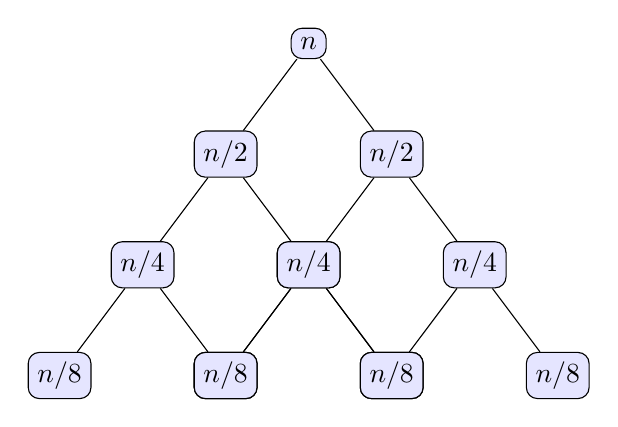
\begin{tikzpicture}[sibling distance=6em, level distance=4em, every node/.style={font=\footnotesize}]
\tikzstyle{every node}=[draw=black,rounded corners,fill=blue!10]
\node {\(n\)}
  child {node {\(n/2\)}
    child {node {\(n/4\)}
      child {node {\(n/8\)}}
      child {node {\(n/8\)}}
    }
    child {node {\(n/4\)}
      child {node {\(n/8\)}}
      child {node {\(n/8\)}}
    }
  }
  child {node {\(n/2\)}
    child {node {\(n/4\)}
      child {node {\(n/8\)}}
      child {node {\(n/8\)}}
    }
    child {node {\(n/4\)}
      child {node {\(n/8\)}}
      child {node {\(n/8\)}}
    }
  };
\end{tikzpicture}
\caption{Recursion Tree of Quick Sort in Best Case (Perfectly Balanced)}
\end{figure}

\paragraph{Observation:}
\begin{itemize}
  \item The recursion depth is \( \log n \) (base 2).
  \item Each level of the tree performs total work proportional to \( n \).
  \item Total time across all levels:
  \[
  n + n + n + \dots + n = n \log n
  \]
  \item Hence, the overall time complexity in the best/average case is:
  \[
  \boxed{T(n) = O(n \log n)}
  \]
\end{itemize}

\subsection*{\textbf{6. Insertion Sort}}
\begin{lstlisting}[language=C++, caption=Insertion Sort]
void insertionSort(vector<int>& arr) {
    for (int i = 1; i < arr.size(); i++) {
        int key = arr[i];
        int j = i - 1;
        while (j >= 0 && arr[j] > key) {
            arr[j + 1] = arr[j];
            j--;
        }
        arr[j + 1] = key;
    }
}
\end{lstlisting}

\subsection*{\textbf{6. Insertion Sort (Analysis)}}

\paragraph{Time Complexity Analysis:}

Insertion Sort builds the sorted array one element at a time. For each element, it is compared with all previous elements and shifted accordingly.

\begin{itemize}
  \item \textbf{Best Case:} The array is already sorted. Each element requires only one comparison:
  \[
  T(n) = \sum_{i=1}^{n-1} 1 = n - 1 \Rightarrow \boxed{O(n)}
  \]

  \item \textbf{Worst Case:} The array is reverse sorted. Every new element is compared with all previous elements and shifted:
  \[
  T(n) = \sum_{i=1}^{n-1} i = \frac{(n-1)n}{2} \Rightarrow \boxed{O(n^2)}
  \]

  \item \textbf{Average Case:} On average, each element is compared with half of the sorted part:
  \[
  T(n) = \sum_{i=1}^{n-1} \frac{i}{2} = \frac{1}{2} \cdot \frac{(n-1)n}{2} = \frac{n(n-1)}{4} \Rightarrow \boxed{O(n^2)}
  \]
\end{itemize}

\paragraph{Space Complexity:}

Insertion Sort is an in-place sorting algorithm.

\[
\boxed{\text{Space Complexity: } O(1)}
\]

\paragraph{Comparison Pattern (TikZ Visualization):}

\begin{figure}[H]
\centering
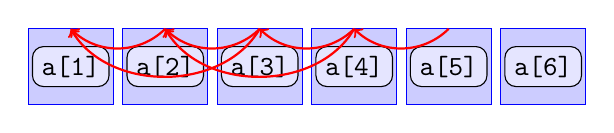
\begin{tikzpicture}[scale=1.2]
\foreach \i in {1,...,6} {
    \filldraw[blue!20, draw=blue] (\i, 0) rectangle (\i+0.9, 0.8);
    \node at (\i+0.45, 0.4) {\texttt{a[\i]}};
}

% Arrows showing comparison path
\draw[->, thick, red] (2.45, 0.8) to[bend left=45] (1.45, 0.8);
\draw[->, thick, red] (3.45, 0.8) to[bend left=45] (2.45, 0.8);
\draw[->, thick, red] (3.45, 0.8) to[bend left=60] (1.45, 0.8);
\draw[->, thick, red] (4.45, 0.8) to[bend left=45] (3.45, 0.8);
\draw[->, thick, red] (4.45, 0.8) to[bend left=60] (2.45, 0.8);
\draw[->, thick, red] (5.45, 0.8) to[bend left=45] (4.45, 0.8);
\end{tikzpicture}
\caption{Comparison pattern in Insertion Sort (Worst Case)}
\end{figure}

\paragraph{Summary:}

\begin{itemize}
  \item \textbf{Best Case:} \(\boxed{O(n)}\)
  \item \textbf{Average Case:} \(\boxed{O(n^2)}\)
  \item \textbf{Worst Case:} \(\boxed{O(n^2)}\)
  \item \textbf{Space Complexity:} \(\boxed{O(1)}\)
\end{itemize}


\subsection*{\textbf{7. Selection Sort}}
\begin{lstlisting}[language=C++, caption=Selection Sort]
void selectionSort(vector<int>& arr) {
    for (int i = 0; i < arr.size() - 1; i++) {
        int minIdx = i;
        for (int j = i + 1; j < arr.size(); j++) {
            if (arr[j] < arr[minIdx]) minIdx = j;
        }
        swap(arr[i], arr[minIdx]);
    }
}
\end{lstlisting}

\subsection*{\textbf{7. Selection Sort (Analysis)}}

\paragraph{Time Complexity Analysis:}

Selection Sort works by repeatedly finding the minimum element from the unsorted part and moving it to the sorted part. It always performs the same number of comparisons regardless of the initial order of the array.

\begin{itemize}
  \item \textbf{Best Case:} Array is already sorted. Still needs to compare all elements to find the minimum.
  \[
  T(n) = \sum_{i=0}^{n-2} (n - i - 1) = \frac{n(n - 1)}{2} \Rightarrow \boxed{O(n^2)}
  \]

  \item \textbf{Worst Case:} Array is in reverse order. Comparisons remain the same.
  \[
  T(n) = \sum_{i=0}^{n-2} (n - i - 1) = \frac{n(n - 1)}{2} \Rightarrow \boxed{O(n^2)}
  \]

  \item \textbf{Average Case:} Same number of comparisons as worst and best cases.
  \[
  \boxed{O(n^2)}
  \]
\end{itemize}

\paragraph{Swap Count:}

Unlike Insertion Sort, Selection Sort performs fewer swaps:
\[
\text{Maximum Swaps: } n - 1 \Rightarrow \boxed{O(n)}
\]

\paragraph{Space Complexity:}

Selection Sort is an in-place sorting algorithm and does not require extra space:
\[
\boxed{\text{Space Complexity: } O(1)}
\]

\paragraph{Comparison Pattern (TikZ Visualization):}

\begin{figure}[H]
\centering
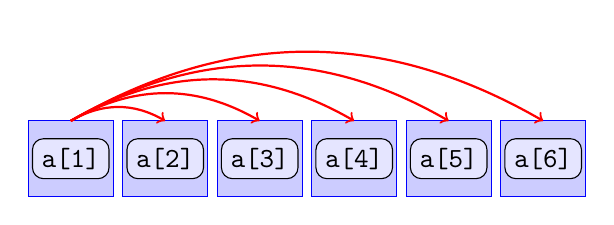
\begin{tikzpicture}[scale=1.2]
\foreach \i in {1,...,6} {
    \filldraw[blue!20, draw=blue] (\i, 0) rectangle (\i+0.9, 0.8);
    \node at (\i+0.45, 0.4) {\texttt{a[\i]}};
}

% Arrows showing selection comparison
\foreach \j in {2,...,6} {
  \draw[->, thick, red] (1.45, 0.8) to[bend left=30] (\j+0.45, 0.8);
}
\end{tikzpicture}
\caption{Selection of the minimum element in each iteration}
\end{figure}

\paragraph{Summary:}

\begin{itemize}
  \item \textbf{Best Case:} \(\boxed{O(n^2)}\)
  \item \textbf{Average Case:} \(\boxed{O(n^2)}\)
  \item \textbf{Worst Case:} \(\boxed{O(n^2)}\)
  \item \textbf{Swap Complexity:} \(\boxed{O(n)}\)
  \item \textbf{Space Complexity:} \(\boxed{O(1)}\)
\end{itemize}


\subsection*{\textbf{8. Heap Sort}}
\begin{lstlisting}[language=C++, caption=Heap Sort]
void heapify(vector<int>& arr, int n, int i) {
    int largest = i;
    int l = 2 * i + 1;
    int r = 2 * i + 2;
    if (l < n && arr[l] > arr[largest]){
        largest = l;
    }
    if (r < n && arr[r] > arr[largest]){
        largest = r;
    }
    if (largest != i) {
        swap(arr[i], arr[largest]);
        heapify(arr, n, largest);
    }
}
void heapSort(vector<int>& arr) {
    int n = arr.size();
    for (int i = n / 2 - 1; i >= 0; i--){
        heapify(arr, n, i);
    }
    for(int i = n - 1; i > 0; i--){
        swap(arr[0], arr[i]);
        heapify(arr, i, 0);
    }
}
\end{lstlisting}

\paragraph{Time Complexity Analysis (Max-Heap):}

\begin{itemize}
  \item \textbf{Heapify operation:} takes \( O(\log n) \).
  \item \textbf{Building heap:} \( O(n) \) (by applying heapify bottom-up).
  \item \textbf{Extracting max (n times):} \( n \cdot O(\log n) = O(n \log n) \).
\end{itemize}

\[
\boxed{\text{Overall Time Complexity (Max-Heap): } O(n \log n)}
\]

\paragraph{Space Complexity:}
Heap Sort is in-place:
\[
\boxed{O(1)}
\]

\paragraph{Tree Diagram (Max-Heap Representation):}

\begin{figure}[H]
\centering
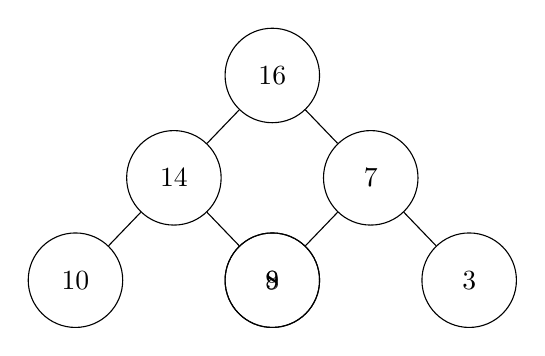
\begin{tikzpicture}[every node/.style={circle,draw,minimum size=1.2cm}, level distance=1.3cm, sibling distance=2.5cm]
\node {16}
  child {node {14}
    child {node {10}}
    child {node {8}}
  }
  child {node {7}
    child {node {9}}
    child {node {3}}
  };
\end{tikzpicture}
\caption{Max-Heap Tree Structure}
\end{figure}

\paragraph{Array Representation (Max-Heap):}

\[
\texttt{[16, 14, 7, 10, 8, 9, 3]}
\]

\paragraph{Tree Diagram (Min-Heap Representation):}

\begin{figure}[H]
\centering
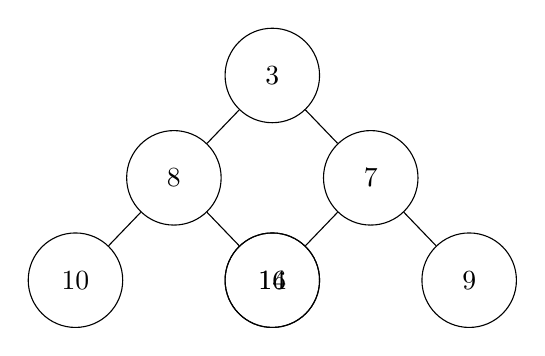
\begin{tikzpicture}[every node/.style={circle,draw,minimum size=1.2cm}, level distance=1.3cm, sibling distance=2.5cm]
\node {3}
  child {node {8}
    child {node {10}}
    child {node {14}}
  }
  child {node {7}
    child {node {16}}
    child {node {9}}
  };
\end{tikzpicture}
\caption{Min-Heap Tree Structure}
\end{figure}

\paragraph{Array Representation (Min-Heap):}

\[
\texttt{[3, 8, 7, 10, 14, 16, 9]}
\]

\paragraph{Time Complexity Analysis (Min-Heap):}
For a min-heap, if we sort in descending order, the time complexity is the same:
\begin{itemize}
  \item \textbf{Heapify:} \( O(\log n) \)
  \item \textbf{Build Heap:} \( O(n) \)
  \item \textbf{n Deletions:} \( O(n \log n) \)
\end{itemize}

\[
\boxed{\text{Overall Time Complexity (Min-Heap): } O(n \log n)}
\]

\paragraph{Summary:}
\begin{itemize}
  \item \textbf{Best Case:} \( O(n \log n) \)
  \item \textbf{Average Case:} \( O(n \log n) \)
  \item \textbf{Worst Case:} \( O(n \log n) \)
  \item \textbf{Space Complexity:} \( O(1) \)
  \item \textbf{Stable:} No
\end{itemize}


\subsection*{\textbf{9. Counting Sort}}
\begin{lstlisting}[language=C++, caption=Counting Sort (Non-negative Integers)]
void countingSort(vector<int>& arr) {
    if (arr.empty()){
        return;
    }
    int maxVal = *max_element(arr.begin(), arr.end());
    vector<int> count(maxVal + 1, 0);
    for (int num : arr){
        count[num]++;
    }
    int idx = 0;
    for (int i = 0; i <= maxVal; i++) {
        while (count[i]-- > 0) arr[idx++] = i;
    }
}
\end{lstlisting}

\paragraph{Time Complexity Analysis:}
Counting Sort assumes all input elements are non-negative integers and works by counting occurrences.

Let \( n \) be the number of elements and \( k \) be the range of input values.

\begin{itemize}
  \item \textbf{Counting frequency:} Takes \( O(n) \).
  \item \textbf{Populating sorted array:} Takes up to \( O(k) \) iterations.
\end{itemize}

\[
\boxed{\text{Time Complexity: } O(n + k)}
\]

\paragraph{Space Complexity:}
Extra space for the count array of size \( k + 1 \):
\[
\boxed{O(k)}
\]

\paragraph{Diagram Representation:}

\begin{figure}[H]
\centering
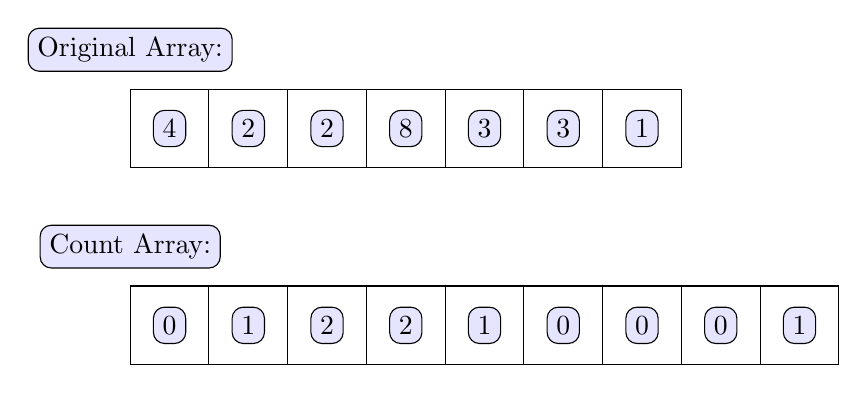
\begin{tikzpicture}[scale=1]
  % Original array
  \node at (0,0.5) {Original Array:};
  \foreach \x/\val in {0/4, 1/2, 2/2, 3/8, 4/3, 5/3, 6/1} {
    \draw (\x,0) rectangle (\x+1,-1);
    \node at (\x+0.5,-0.5) {\val};
  }

  % Count array
  \node at (0,-2) {Count Array:};
  \foreach \x/\val in {0/0, 1/1, 2/2, 3/2, 4/1, 5/0, 6/0, 7/0, 8/1} {
    \draw (\x,-2.5) rectangle (\x+1,-3.5);
    \node at (\x+0.5,-3) {\val};
  }
\end{tikzpicture}
\caption{Counting Sort Diagram: Frequency Count}
\end{figure}

\paragraph{Summary:}
\begin{itemize}
  \item \textbf{Best Case:} \( O(n + k) \)
  \item \textbf{Average Case:} \( O(n + k) \)
  \item \textbf{Worst Case:} \( O(n + k) \)
  \item \textbf{Space Complexity:} \( O(k) \)
  \item \textbf{Stable:} Yes
\end{itemize}

\subsection*{\textbf{10. Radix Sort}}
\begin{lstlisting}[language=C++, caption={Radix Sort (LSD, Non-negative Integers)}]
int getMax(vector<int>& arr) {
    return *max_element(arr.begin(), arr.end());
}
void countingSort(vector<int>& arr, int exp) {
    int n = arr.size();
    vector<int> output(n);
    vector<int> count(10, 0);
    for (int i = 0; i < n; i++) {
        count[(arr[i] / exp) % 10]++;
    }
    for (int i = 1; i < 10; i++) {
        count[i] += count[i - 1];
    }
    for (int i = n - 1; i >= 0; i--) {
        output[count[(arr[i] / exp) % 10] - 1] = arr[i];
        count[(arr[i] / exp) % 10]--;
    }
    for (int i = 0; i < n; i++) {
        arr[i] = output[i];
    }
}
void radixSort(vector<int>& arr) {
    if (arr.size() <= 1) return;
    int max = getMax(arr);
    for(int exp = 1; max / exp > 0; exp *= 10){
        countingSort(arr, exp);
    }
}
\end{lstlisting}

\paragraph{Time Complexity Analysis:}
Radix Sort processes each digit individually using Counting Sort as a stable subroutine.

Let:
\begin{itemize}
  \item \( n \) be the number of elements,
  \item \( k \) be the maximum value in the input,
  \item \( d \) be the number of digits in the maximum number (i.e., \( d = \log_{b} k \), where \( b \) is the base).
\end{itemize}

Each counting sort pass takes \( O(n + b) \) time and we do it for \( d \) digits:
\[
\boxed{\text{Time Complexity: } O(d(n + b)) = O(n \log k)}
\]

For decimal representation (\( b = 10 \)):
\[
\boxed{O(n \cdot \log_{10} k)}
\]

\paragraph{Space Complexity:}
Uses temporary arrays of size \( n \) and \( b \):
\[
\boxed{O(n + b)}
\]

\paragraph{Diagram Representation:}

\begin{figure}[H]
\centering
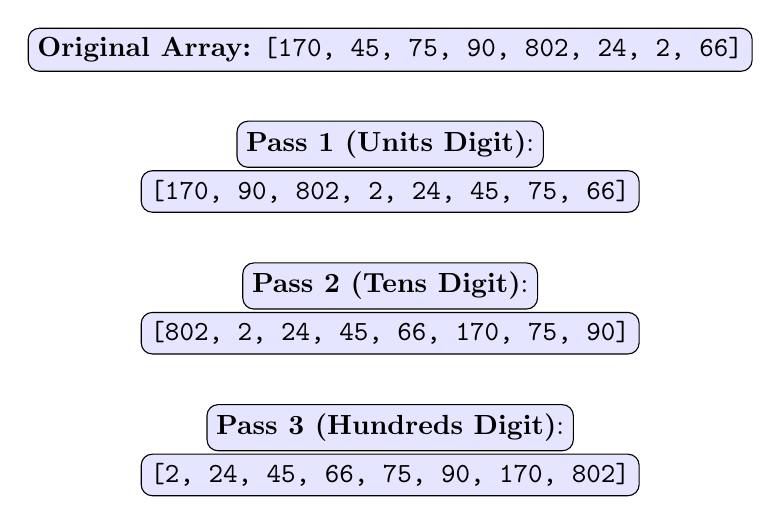
\begin{tikzpicture}[scale=1.2]
\node at (0,1.5) {\textbf{Original Array:} \texttt{[170, 45, 75, 90, 802, 24, 2, 66]}};

\node at (0,0.5) {\textbf{Pass 1 (Units Digit)}:};
\node at (0,0) {\texttt{[170, 90, 802, 2, 24, 45, 75, 66]}};

\node at (0,-1) {\textbf{Pass 2 (Tens Digit)}:};
\node at (0,-1.5) {\texttt{[802, 2, 24, 45, 66, 170, 75, 90]}};

\node at (0,-2.5) {\textbf{Pass 3 (Hundreds Digit)}:};
\node at (0,-3) {\texttt{[2, 24, 45, 66, 75, 90, 170, 802]}};
\end{tikzpicture}
\caption{Radix Sort Progression by Digit Position}
\end{figure}

\paragraph{Summary:}
\begin{itemize}
  \item \textbf{Best Case:} \( O(n \cdot \log_{b} k) \)
  \item \textbf{Average Case:} \( O(n \cdot \log_{b} k) \)
  \item \textbf{Worst Case:} \( O(n \cdot \log_{b} k) \)
  \item \textbf{Space Complexity:} \( O(n + b) \)
  \item \textbf{Stable:} Yes
\end{itemize}

\subsection*{\textbf{11. Bucket Sort}}
\begin{lstlisting}[language=C++, caption=Bucket Sort (Float numbers between 0 and 1)]
void bucketSort(vector<float>& arr) {
    int n = arr.size();
    vector<vector<float>> buckets(n);
    for (int i = 0; i < n; i++) {
        int idx = n * arr[i];
        buckets[idx].push_back(arr[i]);
    }
    for (int i = 0; i < n; i++){
        sort(buckets[i].begin(), buckets[i].end());
    }
    int idx = 0;
    for (int i = 0; i < n; i++) {
        for (float val : buckets[i]) {
            arr[idx++] = val;
        }
    }
}
\end{lstlisting}

\paragraph{Time Complexity Analysis:}
Bucket Sort distributes elements into buckets and sorts them individually.

Let:
\begin{itemize}
  \item \( n \) be the number of elements,
  \item \( k \) be the number of buckets (commonly \( k = n \)).
\end{itemize}

Assuming uniform distribution and insertion sort inside each bucket:

\begin{itemize}
  \item \textbf{Distribute into buckets:} \( O(n) \)
  \item \textbf{Sort each bucket:} Expected \( O(n) \) if elements are uniformly distributed
\end{itemize}

\[
\boxed{\text{Expected Time Complexity: } O(n)}
\]

\textbf{Worst-case:} When all elements fall into a single bucket, leading to:
\[
\boxed{O(n^2)}
\]

\paragraph{Space Complexity:}
Additional space for buckets:
\[
\boxed{O(n)}
\]

\paragraph{Diagram Representation:}

\begin{figure}[H]
\centering
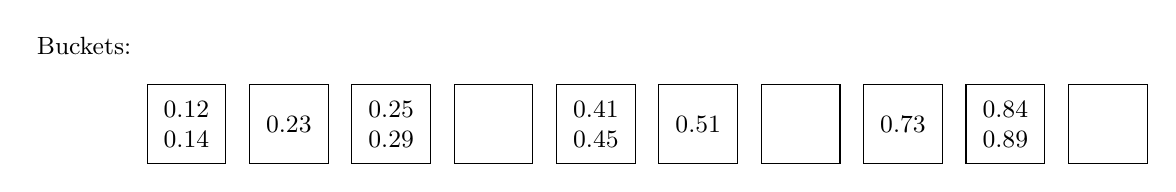
\begin{tikzpicture}[scale=1, every node/.style={font=\small}]
\node at (-0.8,0.5) {Buckets:};

% Buckets
\foreach \x/\val in {0/{0.12\\0.14}, 1/{0.23}, 2/{0.25\\0.29}, 3/{}, 4/{0.41\\0.45}, 5/{0.51}, 6/{}, 7/{0.73}, 8/{0.84\\0.89}, 9/{}} {
    \draw (\x*1.3,0) rectangle (\x*1.3+1, -1);
    \node[align=center] at (\x*1.3+0.5, -0.5) {\val};
}
\end{tikzpicture}
\caption{Bucket Sort Buckets with Sorted Values}
\end{figure}

\paragraph{Summary:}
\begin{itemize}
  \item \textbf{Best Case:} \( O(n) \)
  \item \textbf{Average Case:} \( O(n) \)
  \item \textbf{Worst Case:} \( O(n^2) \)
  \item \textbf{Space Complexity:} \( O(n) \)
  \item \textbf{Stable:} Depends on internal sort (e.g., insertion sort = stable)
\end{itemize}

\subsection*{\large \textbf{6. Highlighting Function Notations}}

We often express the dominating term of a function using color to emphasize its impact. For example, consider:
\[
\mathbf{f(n) = \textcolor{blue}{n^2} + 3n + 2}
\]
For large \( n \), the term \(\textcolor{blue}{n^2}\) dominates, hence:
\[
f(n) = \Theta(\textcolor{blue}{n^2})
\]
This shows that lower-order terms and constants are ignored in asymptotic analysis.